\chapter{修士作品 《Grasp(er)》}
\label{about_grasper}
本章では、修士作品《Grasp(er)》の概要と、その制作プロセスを説明する。

\section{作品概要}
\begin{figure}[H]
  \centering
  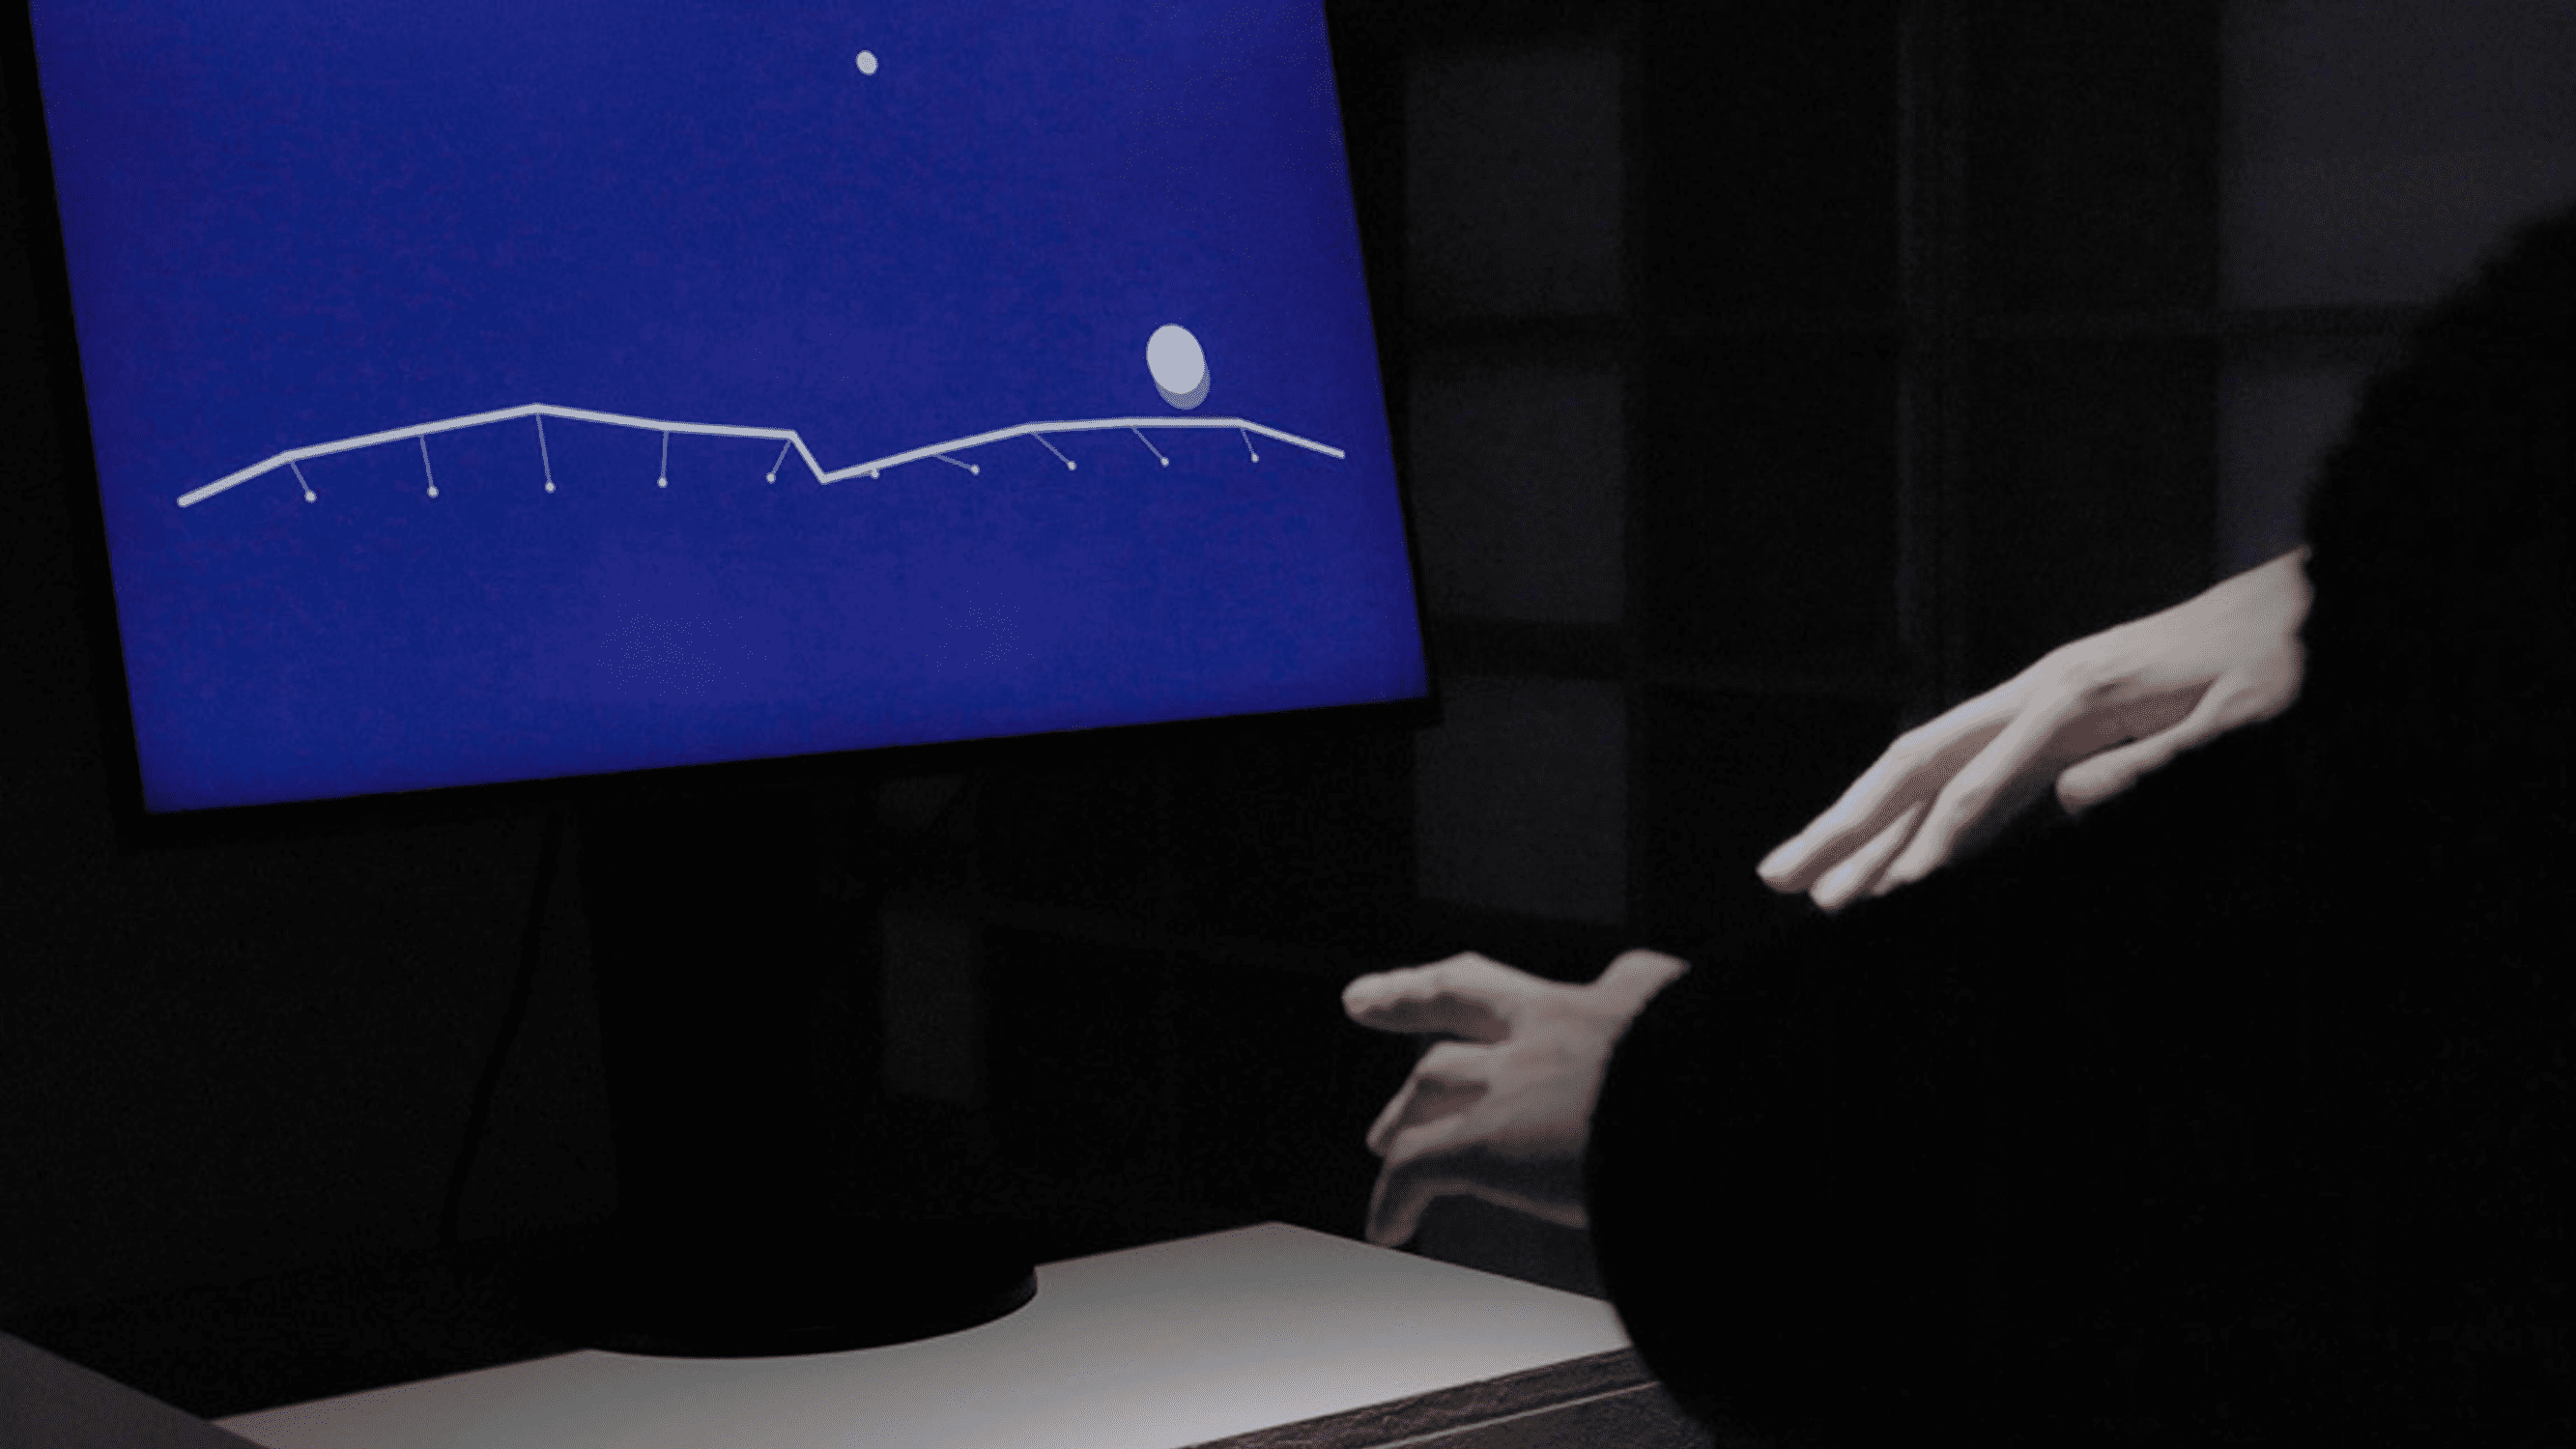
\includegraphics[width=15cm]{img/thumbnail.png}
  \caption{修士作品《Grasp(er)》}
  \label{grasper}
\end{figure}

《Grasp(er)》は、「Familiar / Strange」と「Relation」という二つから構成された作品群である。手の形が大きく変化したり、その変化した手指を使った細かな操作が求められる中で芽生える、身体の他者性に対する注目を扱った作品である。

最初はうまくいかず「もどかしさ」を感じながらも、試行錯誤や意識的な身体動作を行う期間を経て折り合いをつけていく過程に、「変化」が起こる。高度な道具の能力を享受するだけでなく、\textit{grasp}を通して、人が能力を身につけるという側面に着目して、作品名を《Grasp(er)》とした。

以下では、本作を構成する2つの作品について説明する。

% これらに共通するのは、\textit{grasp}の中で個人が目的意識や興味を抱くことで、\textit{grasp}が連鎖的に生じることである。

% 制作者は「このようなことをしてほしい」という行為の中身を設計せず、体験する個人がその中で次々と注目する対象を見出すことによって、個人が行為を創造していくことを目指している。このため、「手指の構造や、手指を取り巻く環境を変化させることで、手指の運動に注目する構造」を作ることに取り組んだ。このときの「注目」が起点となって\textit{grasp}の期間が生じるが、その先々で起こる体験は個人に委ねられ、明示的な目的は設定されていない。

\subsection*{Familiar / Strange}
\begin{figure}[H]
  \centering
  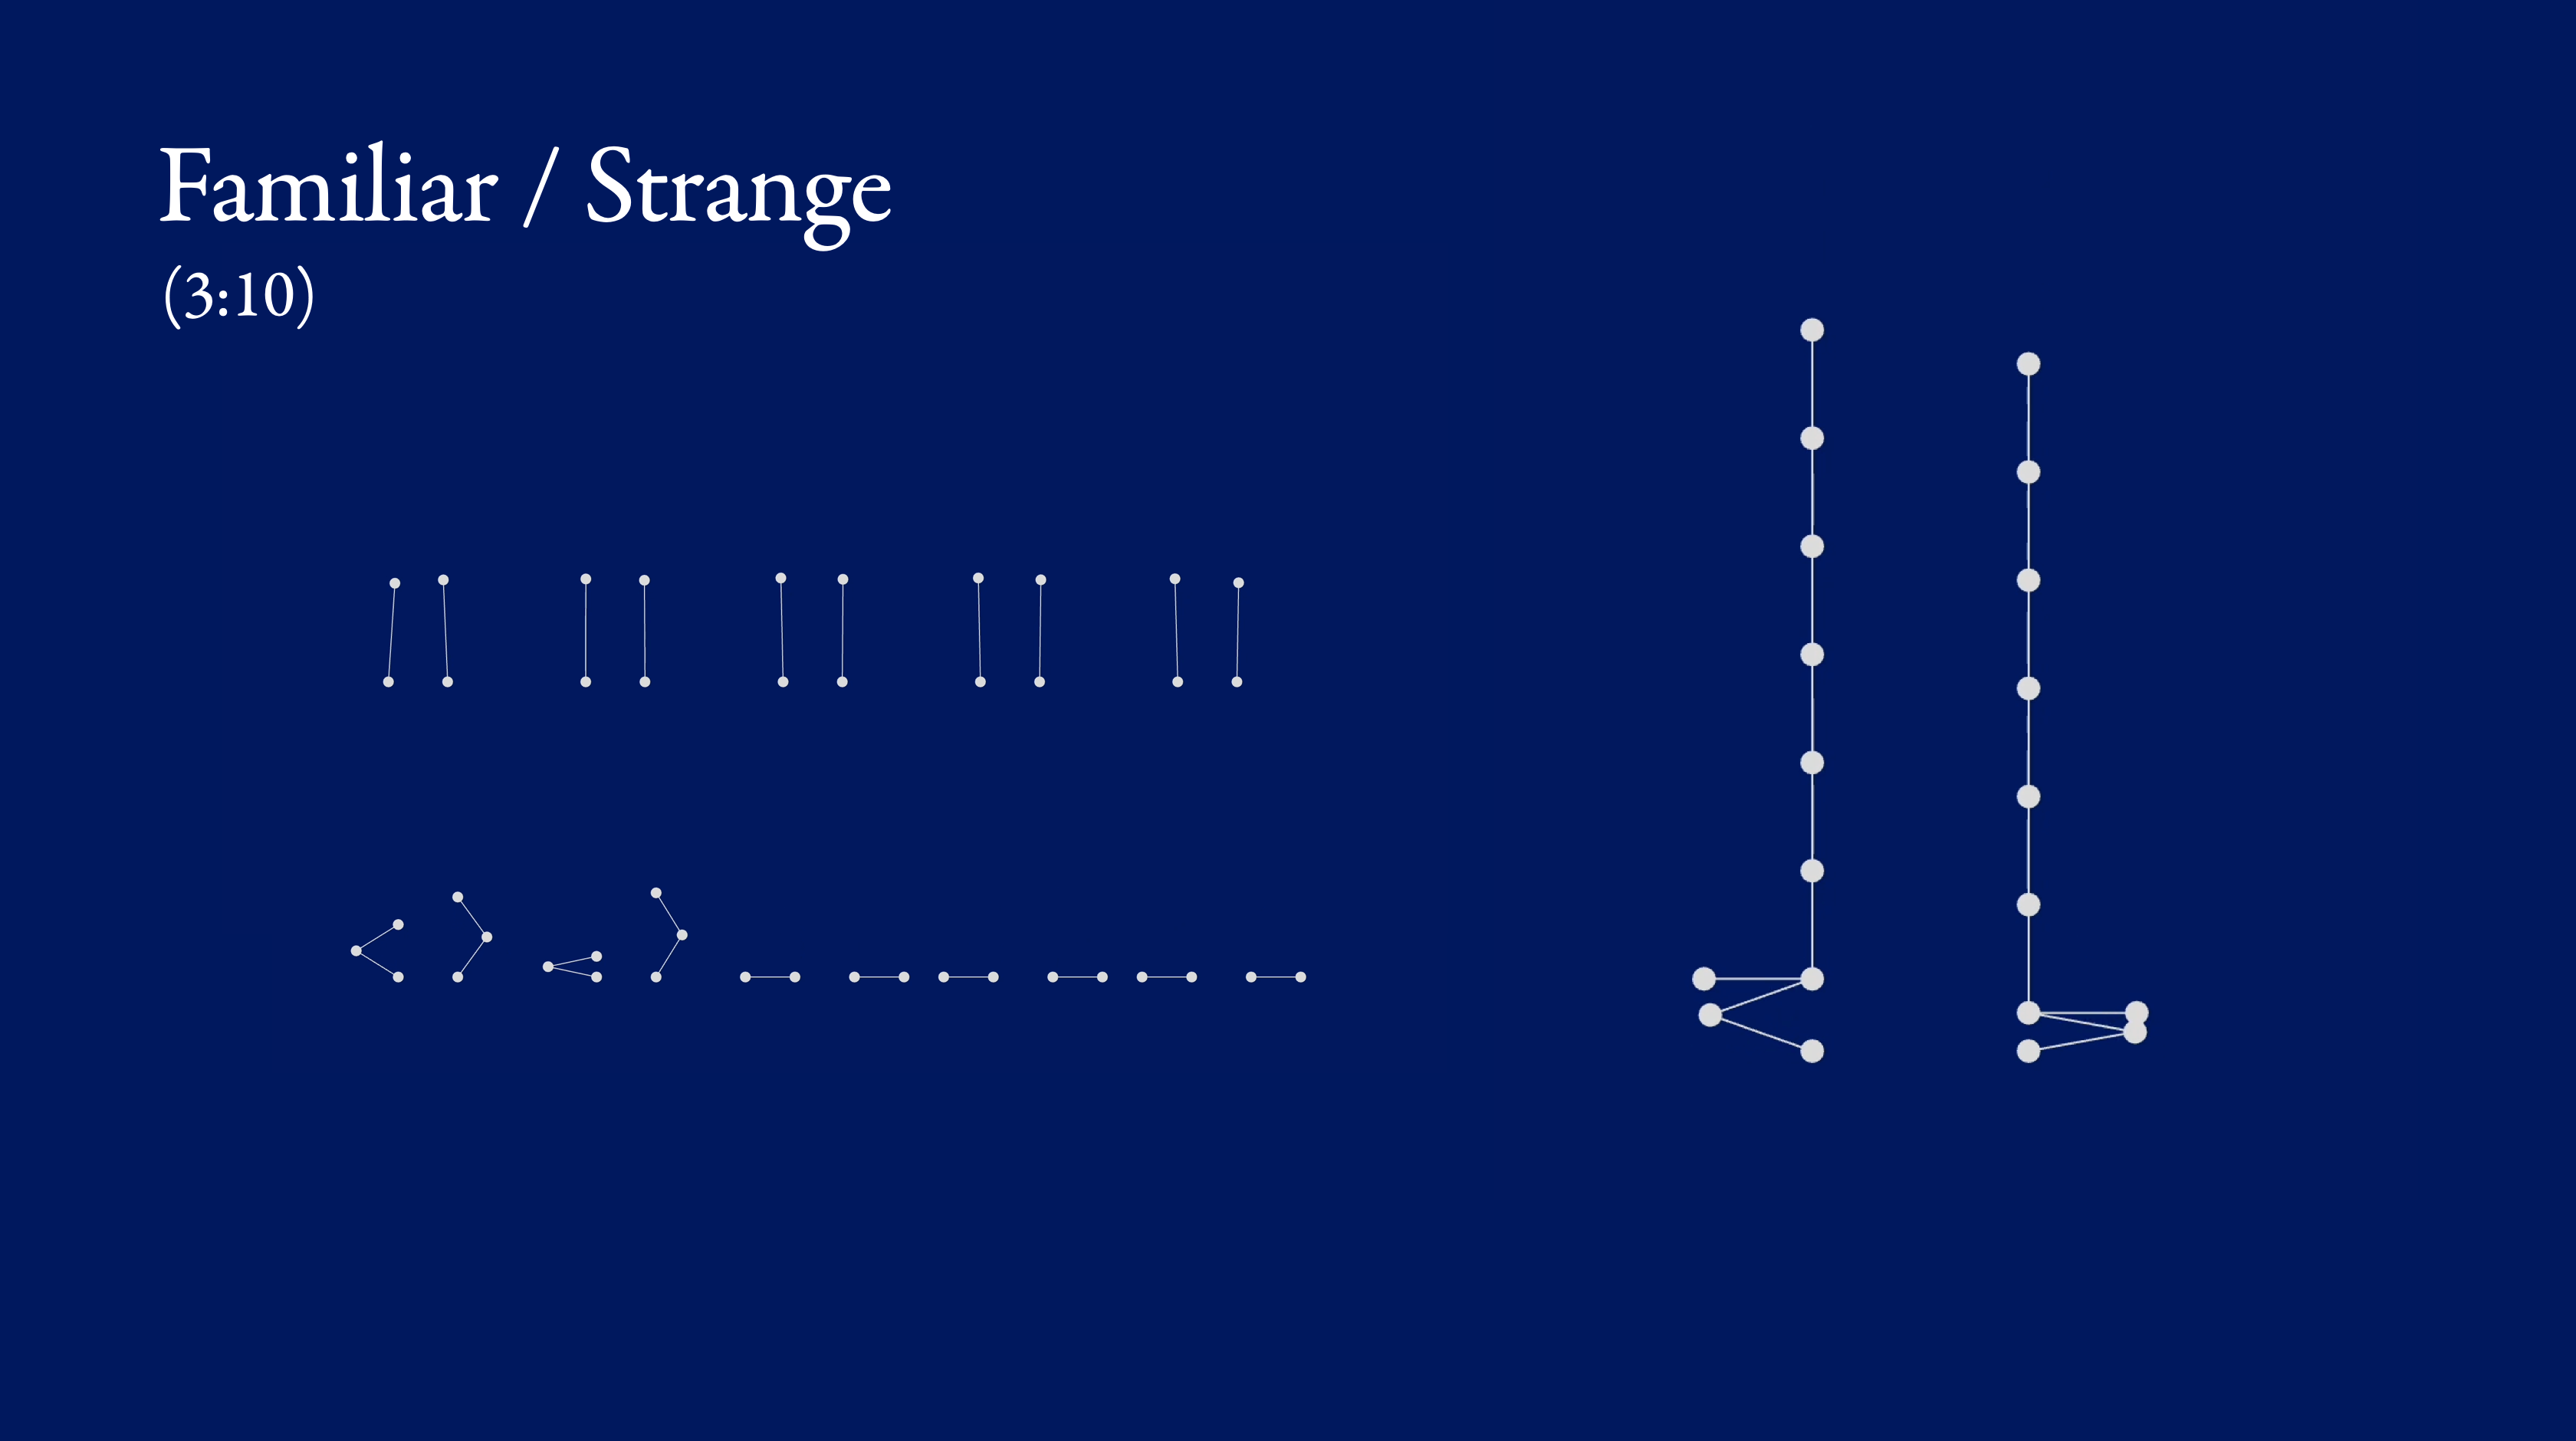
\includegraphics[width=15cm]{img/fs-02.png}
  \caption{Familiar / Strange}
  \label{fig:familiar_strange}
\end{figure}
「Familiar / Strange」は、手指の配置や関節の数・位置が次々と変化していく作品で、手の運動に対する再注目が起きることを目指している。作品は最初、手の形がそのまま現れた状態から開始し、指の並びや関節の配置の変化が起きる。一本一本の指がくの字の形をして積み上げられる様子をピークに、逆順に変化が巻き戻され、再び元の手の形に戻るという、3分10秒で1ループの構造となっている。


変換の過程は、イージングやゴム紐が切れた時のような振動を伴う動きによって補完される。シーン遷移を説明する図を以下に示す。
\begin{figure}[H]
  \centering
  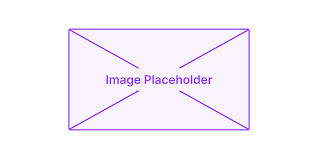
\includegraphics[width=15cm]{img/placeholder.png}
  \caption{Familiar / Strangeにおけるシーン遷移}
  \label{fig:diagram_familiar_strange}
\end{figure}

\subsection*{Relation}
\begin{figure}[H]
  \centering
  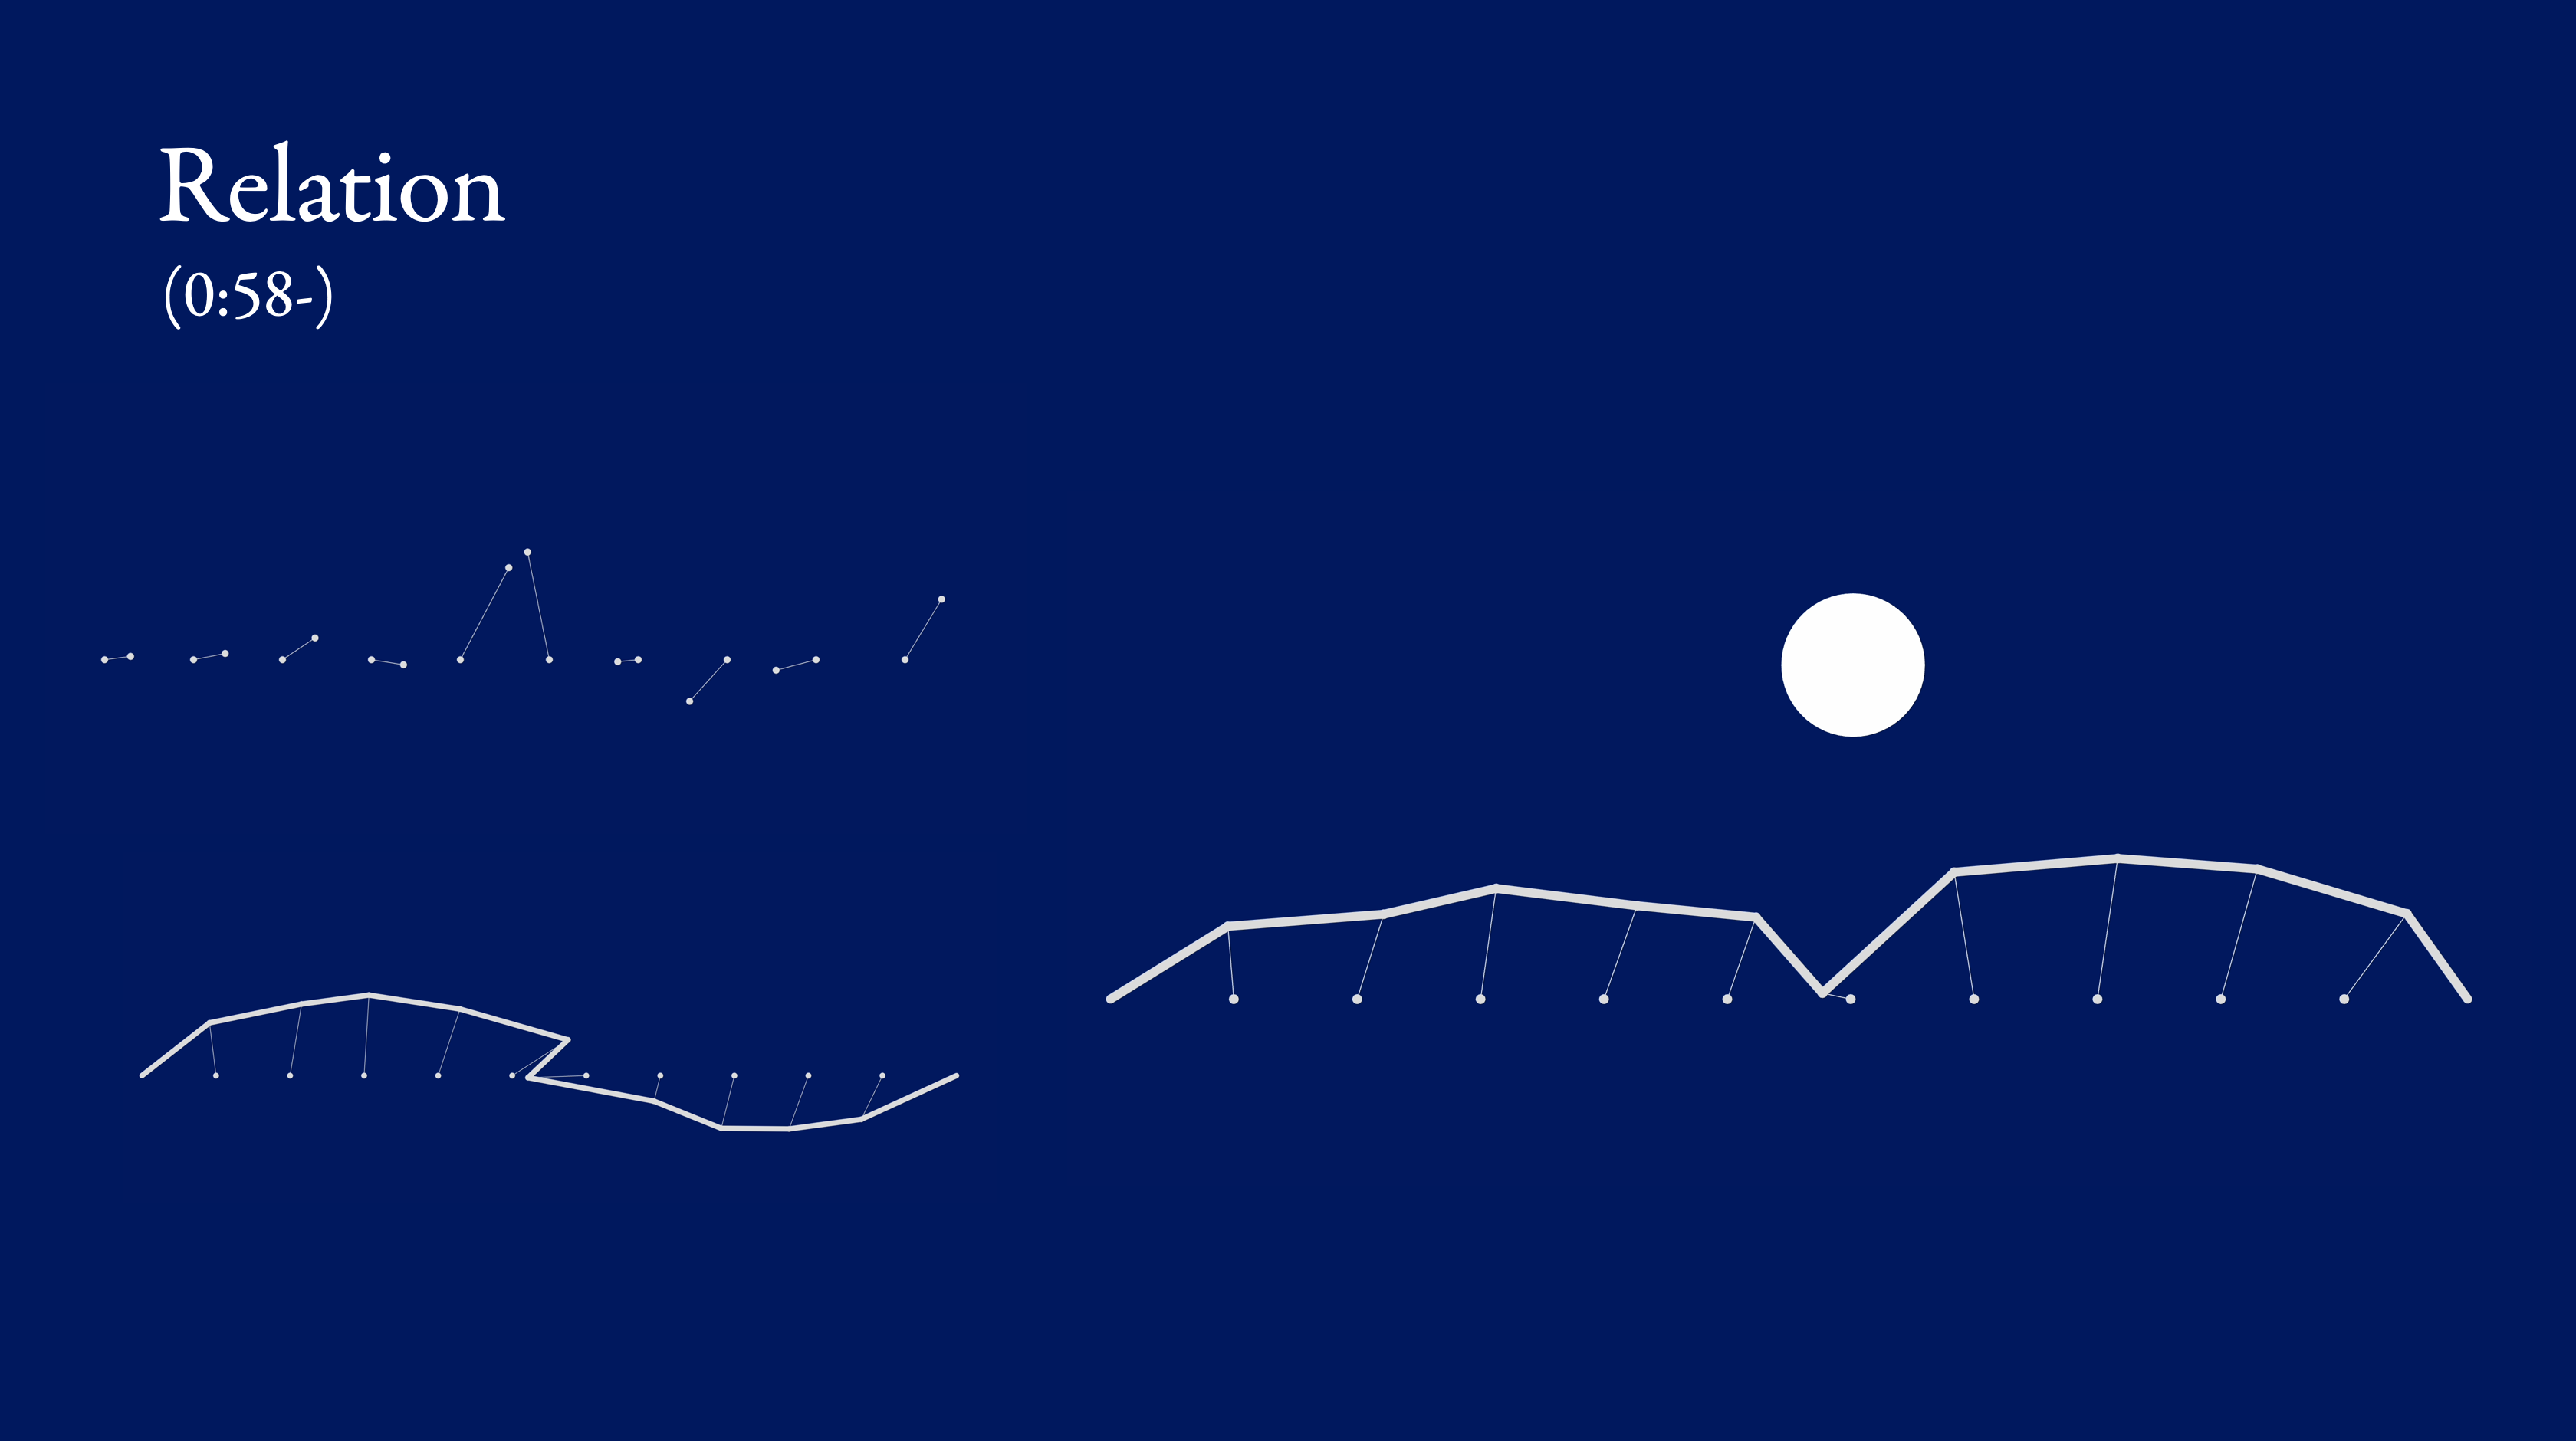
\includegraphics[width=15cm]{img/relation.png}
  \caption{Relation}
  \label{fig:relation}
\end{figure}
「Relation」は、変化した手指を取り巻く関係が次々と変化していく作品で、手と直接的に制御できないボールの関係性におけるGraspに焦点を当てている。1つ目の作品と同様、最初は手が表示された状態から始まり、段階的に並び替えられた手指を覆う皮膜が現れ、ボールが現れる。最後はマトが現れ、的を取るたびにボールの大きさが小さくなり、3つ連続して取ると、皮膜は消え、再び元の手の形に戻る。

トラッキングされた手指の位置が、手首から指ごとに分割され、左端から右へ、左手の小指から親指、そして右手の親指から小指の順に整列される。しばらくすると、指先以外の運動が捨象され、残された指先を結ぶ線が現れる。ここで、現れた線によって再び全ての指が1つのまとまりとして統合されることになるが、その線は後に現れるボールに対して衝突判定が適用される、新しい構造の手指を覆う皮膜のような機能を有する。皮膜のある領域を外れるとボールは落下するが、そのあとは再び画面の中央にボールが出現する。

さらに一定時間が経過すると、皮膜の上方に白い点:マトが現れる。マトに対してボールを当てると、ボールは一回り小さくなり、ボールを落とさずに合計3回マトに当てることでボールは消失し、皮膜が現れるときと逆の順序を辿って画面の中の手は再びもとの形状に戻る。

\section{\textit{grasp}による作品体験の仮説}
\label{nerai}
本作品におけるねらいと学内での作品審査の作品体験の様子を踏まえて、本作について\textit{grasp}の観点から仮説を立てる。

\subsection*{Familiar / Strange}
本作における主な注意は、モーフィングを起点に生じる「親和性が失われる感覚」である。最初、手指が鏡合わせのように表示された状態から始まり、ゆっくりと指一本一本の単位で分割されていく。その瞬間に、見慣れていたはずの手指の動きが見慣れないものに感じられ、\textit{grasp}が生じる。2つ目の作品と比べると、ゆっくりとしたテンポで手指の形状が変化する。そのためしばらくすると変化した手指の構造に慣れ、またそれが別の形に変化していく際に再び親和性の失われる感覚が生じると考える。

この変化をFelsの分類から捉えると、手指の変換が起点となってIntimacyが低下し、「確認」の動作として\textit{response}や\textit{contemplation}が生じる。しばらく手を動かしている中で要領が掴めてくると、ControlやBelongingが生まれ、再び別の形でIntimacyの生じる体験になると考える。

また、変換のピークであるバネ状に指の動きが連結されたときには、はじめて指の動きが相互に干渉するようになり複雑度が増す。そのため注意を向ける対象が増え、より長く\textit{grasp}が生じるのではないかと考えた。

\begin{figure}[H]
  \centering
  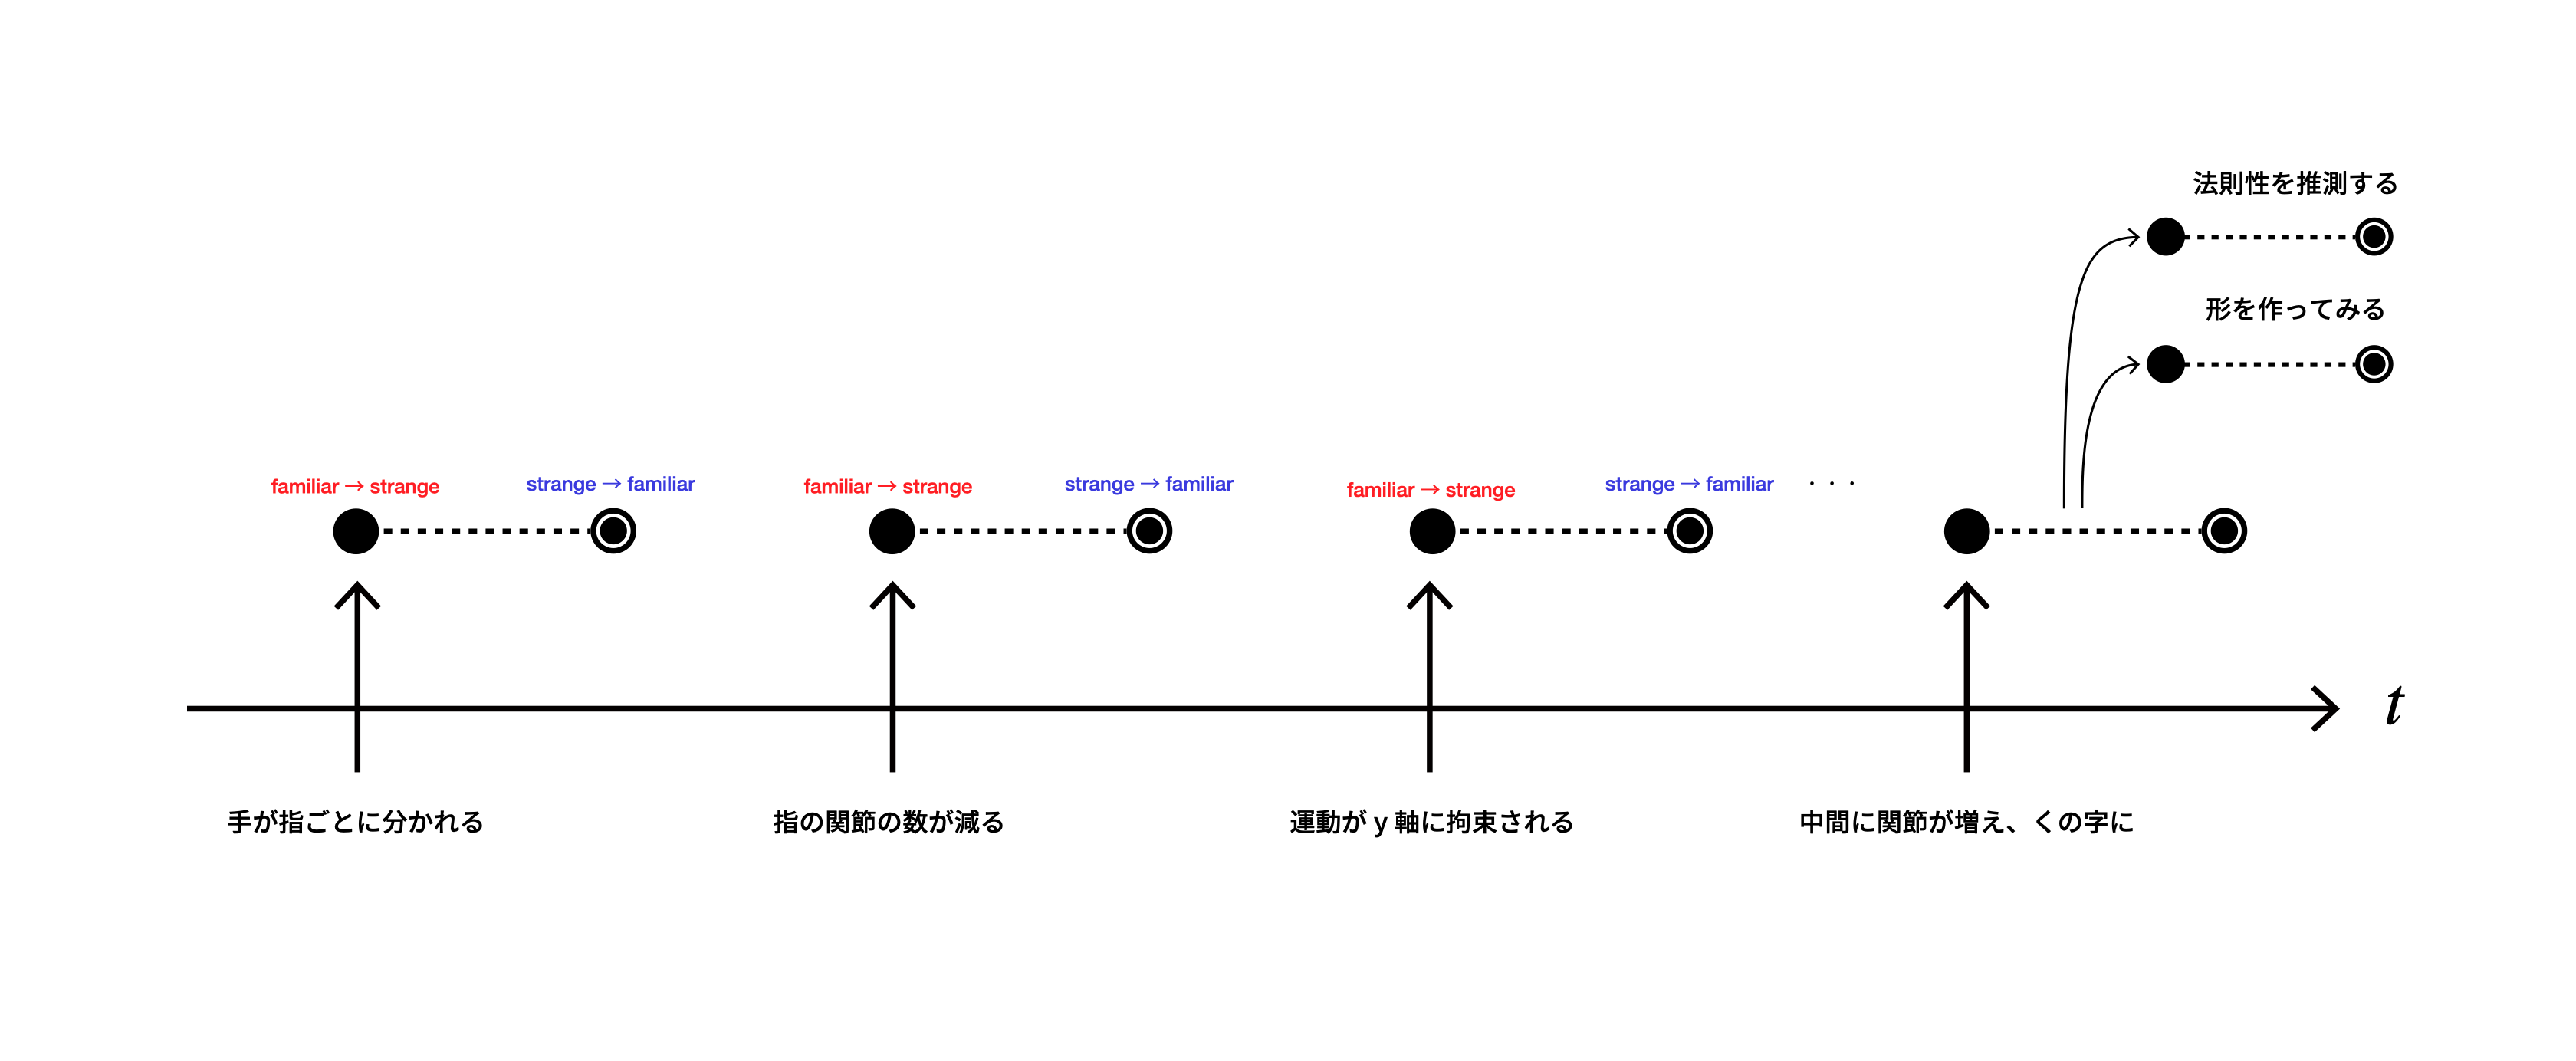
\includegraphics[width=15cm]{img/grasp_familiar_strange.png}
  \caption{Familiar / Strangeにおける\textit{grasp}}
  \label{fig:grasp_familiar_strange}
\end{figure}

\subsection*{Relation}
この作品は、1つめの「Familiar / Strange」と異なり、構造が変化した手指と、ボールという直接的に動かすことができない対象との関係性に注意が向けられることをねらいとした。
ただし先に指摘したように、ボールと手の関係に注意が向いた途端、手指に感じる違和感や注意は向きづらくなる。さらに、マトが現れると、さらにその目的意識は強固になると考えた。これまでの展示の様子から、ボールと手指だけの関係性であっても、まずは飛ばしてみる、転がしてみる、落とさないように気を付けるといった目的意識を設定しやすい。その一方で、手指のみの状態から手指とボールとの関係性に切り替わったときと同様に、マトが出現することがそうした注意を不可視にしてしまうことがこれまでの展示の中で見受けられた。

そのため、手指の変換、皮膜の出現、ボールの出現、そしてマトの出現は、それぞれタイミングを分けて出力するように調整した。本作はダイナミックな構造の切り替わりこそ少ないが、手指を取り巻く関係性が次々に変化する作品として構成された。そうすることで、それぞれの関係性において異なる注意が生じ、段階的に目的意識が強固になっていくことで、「マトにボールを当てる」という強い目的意識とその達成のための試行錯誤を通して、強い一体感が生じるのではないかと考えた。

\begin{figure}[H]
  \centering
  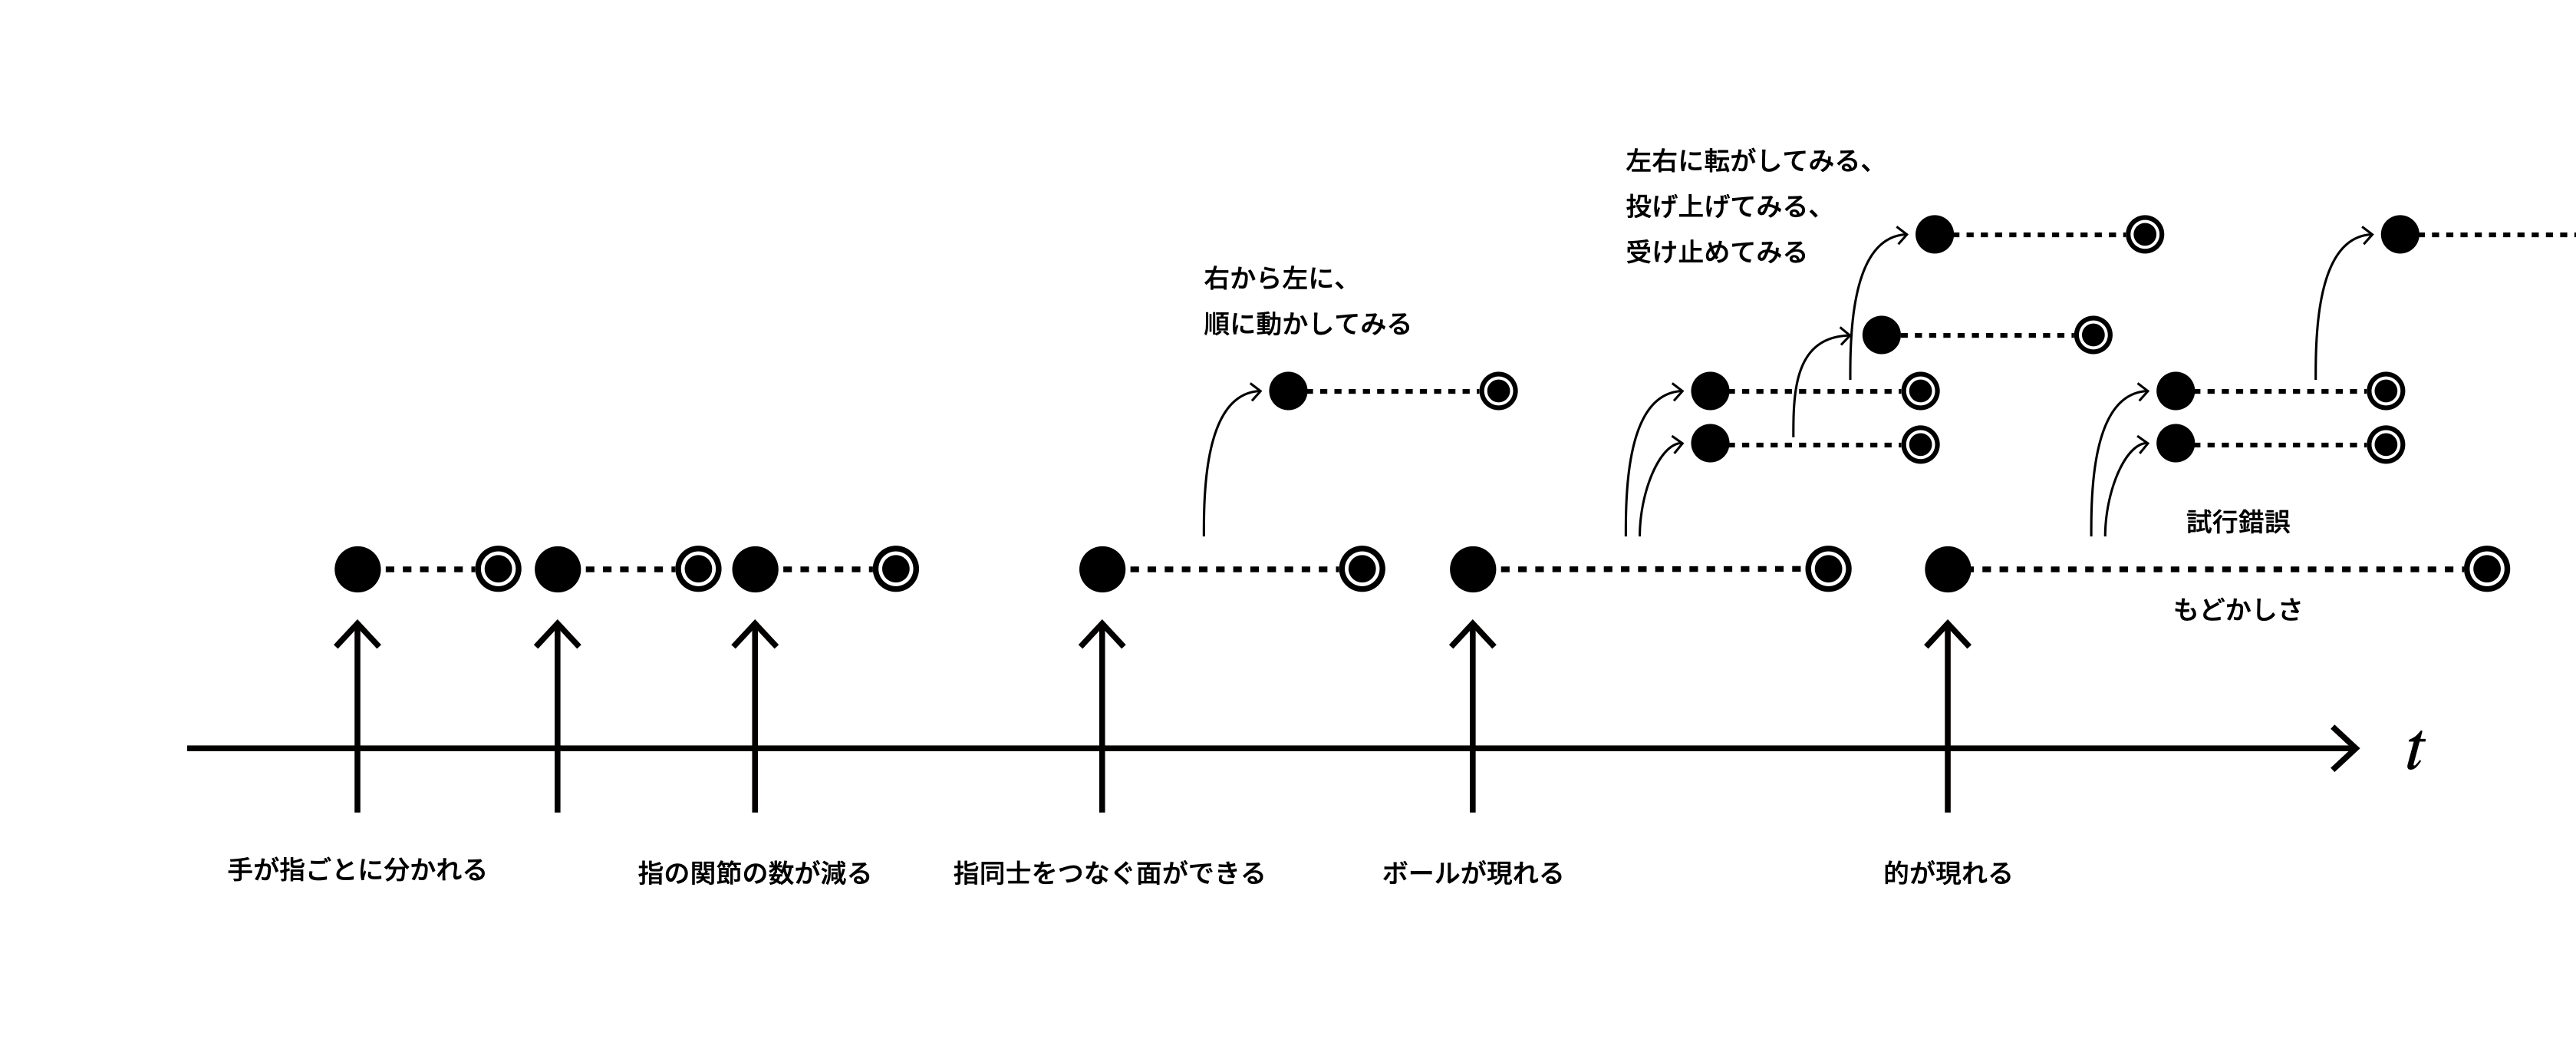
\includegraphics[width=15cm]{img/grasp_relation.png}
  \caption{Relationにおける\textit{grasp}}
  \label{fig:grasp_relation}
\end{figure}

% \textit{grasp}には二つの性質がある。一つは、時間幅が注意を向けている対象によって、長い場合と短い場合があることである。目的意識が芽生えてからスムーズに操作できるようになる場合、'reach'から'manipulate'が近く、\textit{grasp}は短い、すなわち直感的で使いやすいものとして経験される。その一方、目的意識が芽生えてから試行錯誤を伴い、習熟に長い期間を要する場合、\textit{grasp}は長く、もどかしさを経験し、操れるようになった時に達成感を経験する。\\

% 二つ目に、\textit{grasp}の過程で他のことに対する意識が次々と芽生えることがある。具体的には「やってみるまでわからない」といった経験や、物事に対する解像度が高まる中で、当初とは異なる意識が芽生える状況に相当する。\\

% このコンセプトを展開し、「試行錯誤の余地」を設計することを目指したのが、修士作品《Grasp(er)》である。この作品では、\textit{grasp}を経験する中で、個人による創造的な活動が生まれ、\textit{grasp}という動作を行っているのではなく、そこに'er'の接尾辞がついた'Grasper'であると名付けた。

\section{ライブラリの開発}
本作品を構成するにあたり、基本的な関数をまとめたライブラリを開発した。ライブラリには、円滑に体験するための補完処理を実装している。
具体的には、ガウシアンフィルターによる平滑化処理、トラッキングが途切れた際の例外処理の2つである。

\subsection{ガウシアンフィルターによる平滑化処理}
推定精度の問題から、モデルより推定される姿勢情報をそのまま出力すると、手指を動かしていなくても小刻みに振動したり、一時的なフレームレートの低下に起因してスムーズに動作していないように感じることがある。\\
そこで、体験者にフィードバックする際に使用する姿勢情報は、前後2フレーム分のフレーム情報にガウシアンフィルターを適用した平滑化処理を実装している。ただし、トラッキングが開始した直後は5フレーム分のフレーム情報を使用することができないため、この場合は取得できる限りのフレーム情報を用いて同じ処理を行なっている。そのため以下では、各フレーム情報に対する重みづけと、それを用いて体験者に提示される姿勢情報を求める上での一般式を示す。
モデルより推定された最新の姿勢情報を\(P_{n}\)、出力されている姿勢情報を\(S\)とすると、
  % 平滑化フレーム S の定義
  \begin{equation}
    S = \sum_{i=-2}^{2} w_i' \cdot P_{n+i}
    \end{equation}

ここで、\(w_i'\)は正規化されたガウシアンフィルタの重みを表す。正規化前の重み\(w_i\)は、
\begin{equation}
  w_i = \frac{1}{\sqrt{2\pi}\sigma} e^{-\frac{i^2}{2\sigma^2}}
  \end{equation}

正規化された重み\(w_i'\)は、
  % 重みの正規化
  \begin{equation}
  w_i' = \frac{w_i}{\sum_{j=-2}^{2} w_j}
  \end{equation}
と表現される。
この処理のため、最良時で60fps程度で取得される姿勢情報は、慢性的に0.3sほどの遅延を伴って体験者にフィードバックされることになる。

\subsection{トラッキングが途切れた際の例外処理}
体験時、環境光や、手指を動かす範囲や速度の関係から、トラッキングが途切れることがある。素早い動きをしている最中に1フレームでも途切れると円滑に体験することができないため、この時は例外的に、トラッキングが途切れる直前のフレーム情報で失われたフレーム情報を埋め合わせる処理を実装した。また、トラッキングが途切れていることに起因する不快感は、本作品の体験外の問題なので、手指の動きがトラッキングできていない状態を視覚的にフィードバックするため、トラッキング不能時に塗りつぶしを透過する視覚効果を実装した(\ref{fig:track_true}, \ref{fig:track_false})。

\begin{figure}[htbp]
  \begin{minipage}[b]{0.5\linewidth}
    \centering
    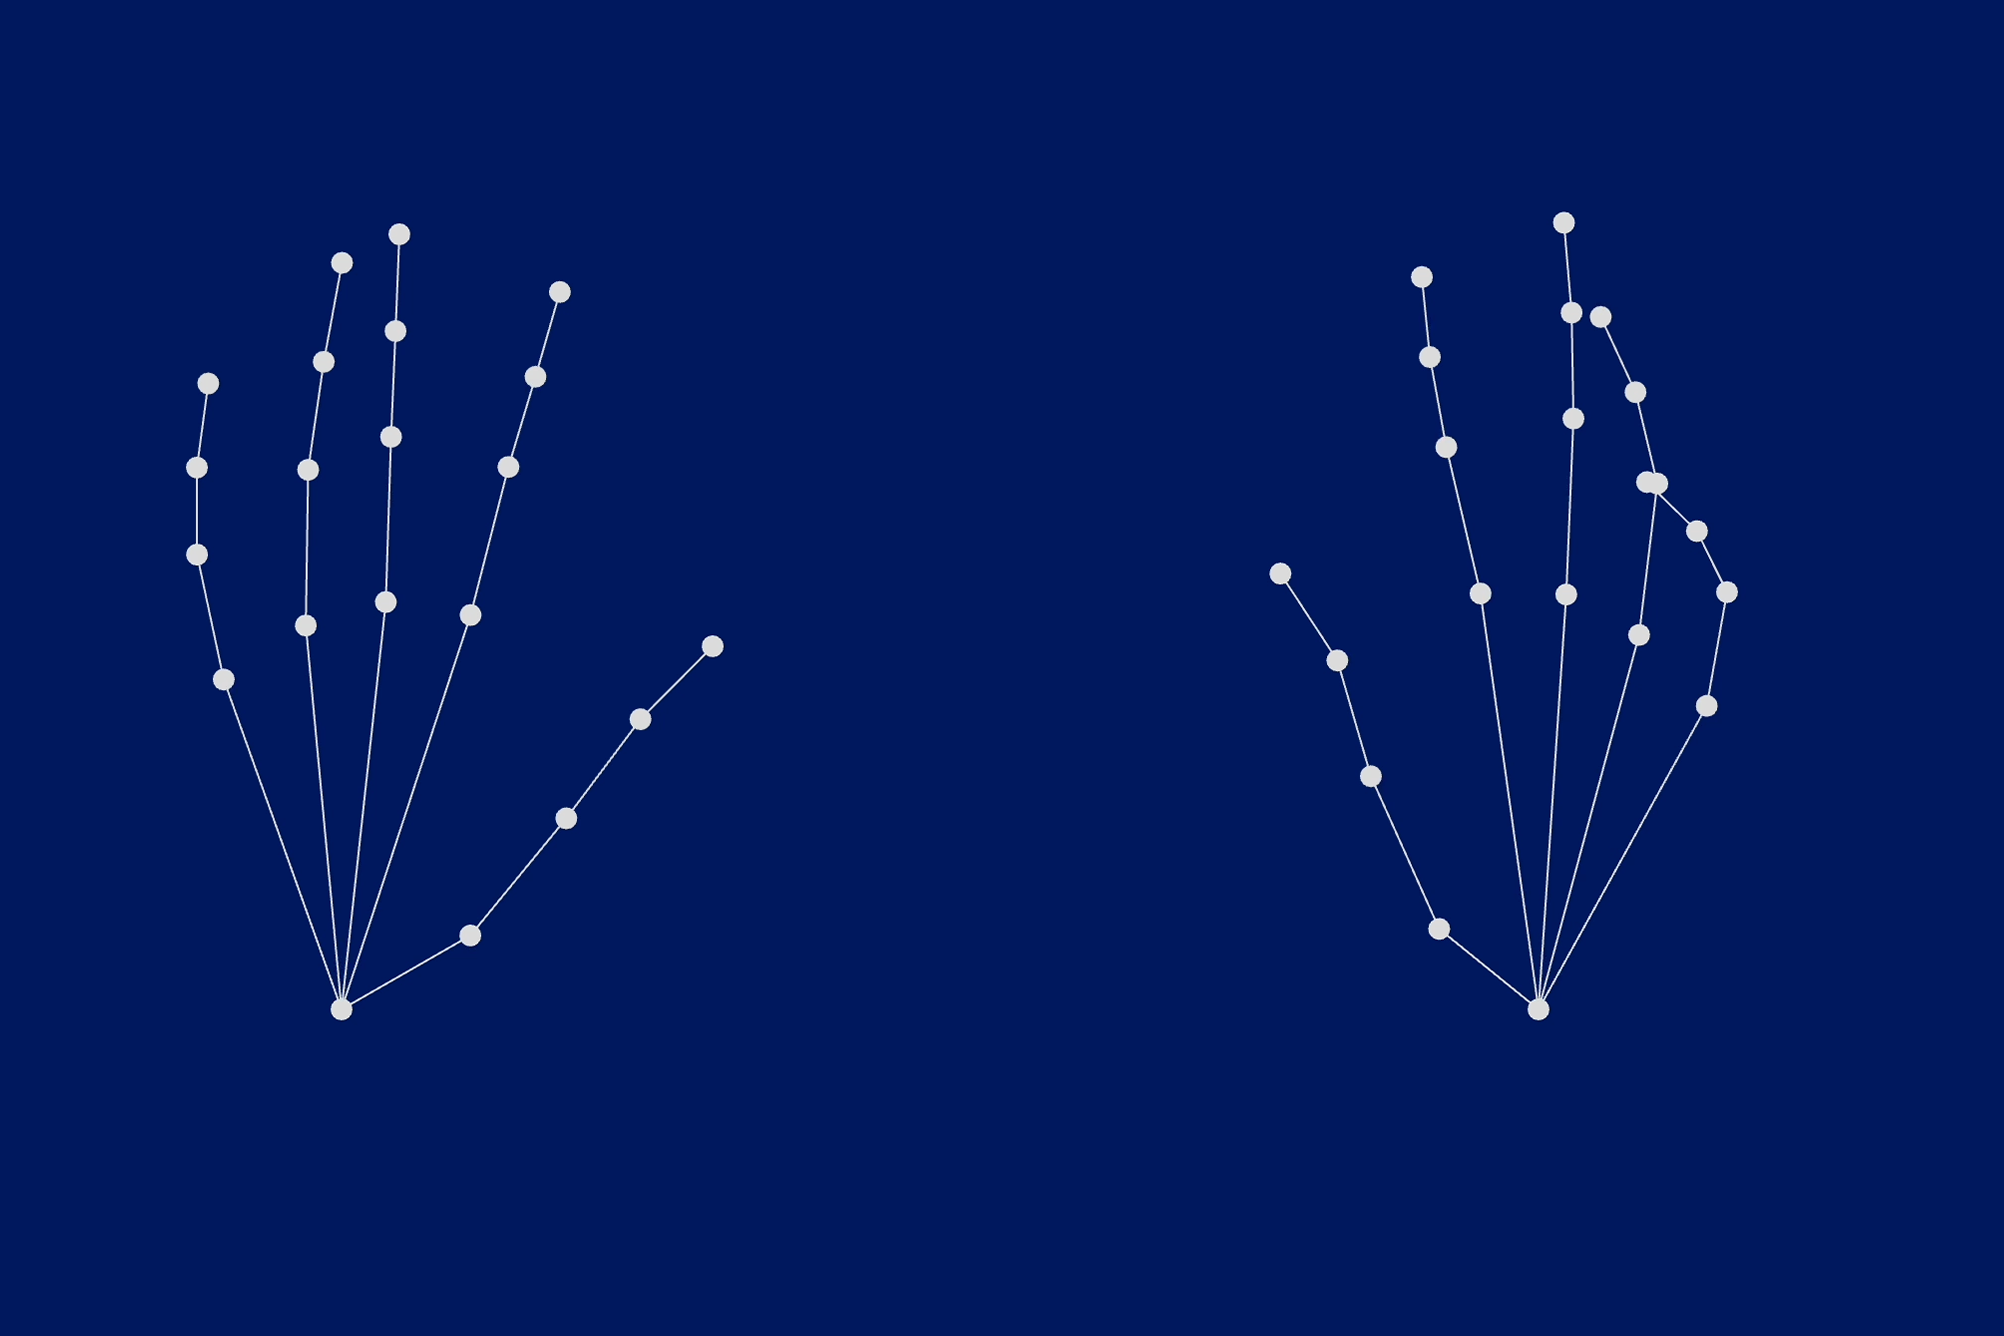
\includegraphics[keepaspectratio, width=7cm]{img/track_true.png}
    \caption{トラッキングが正常にできているとき}
    \label{fig:track_true}
  \end{minipage}
  \begin{minipage}[b]{0.5\linewidth}
    \centering
    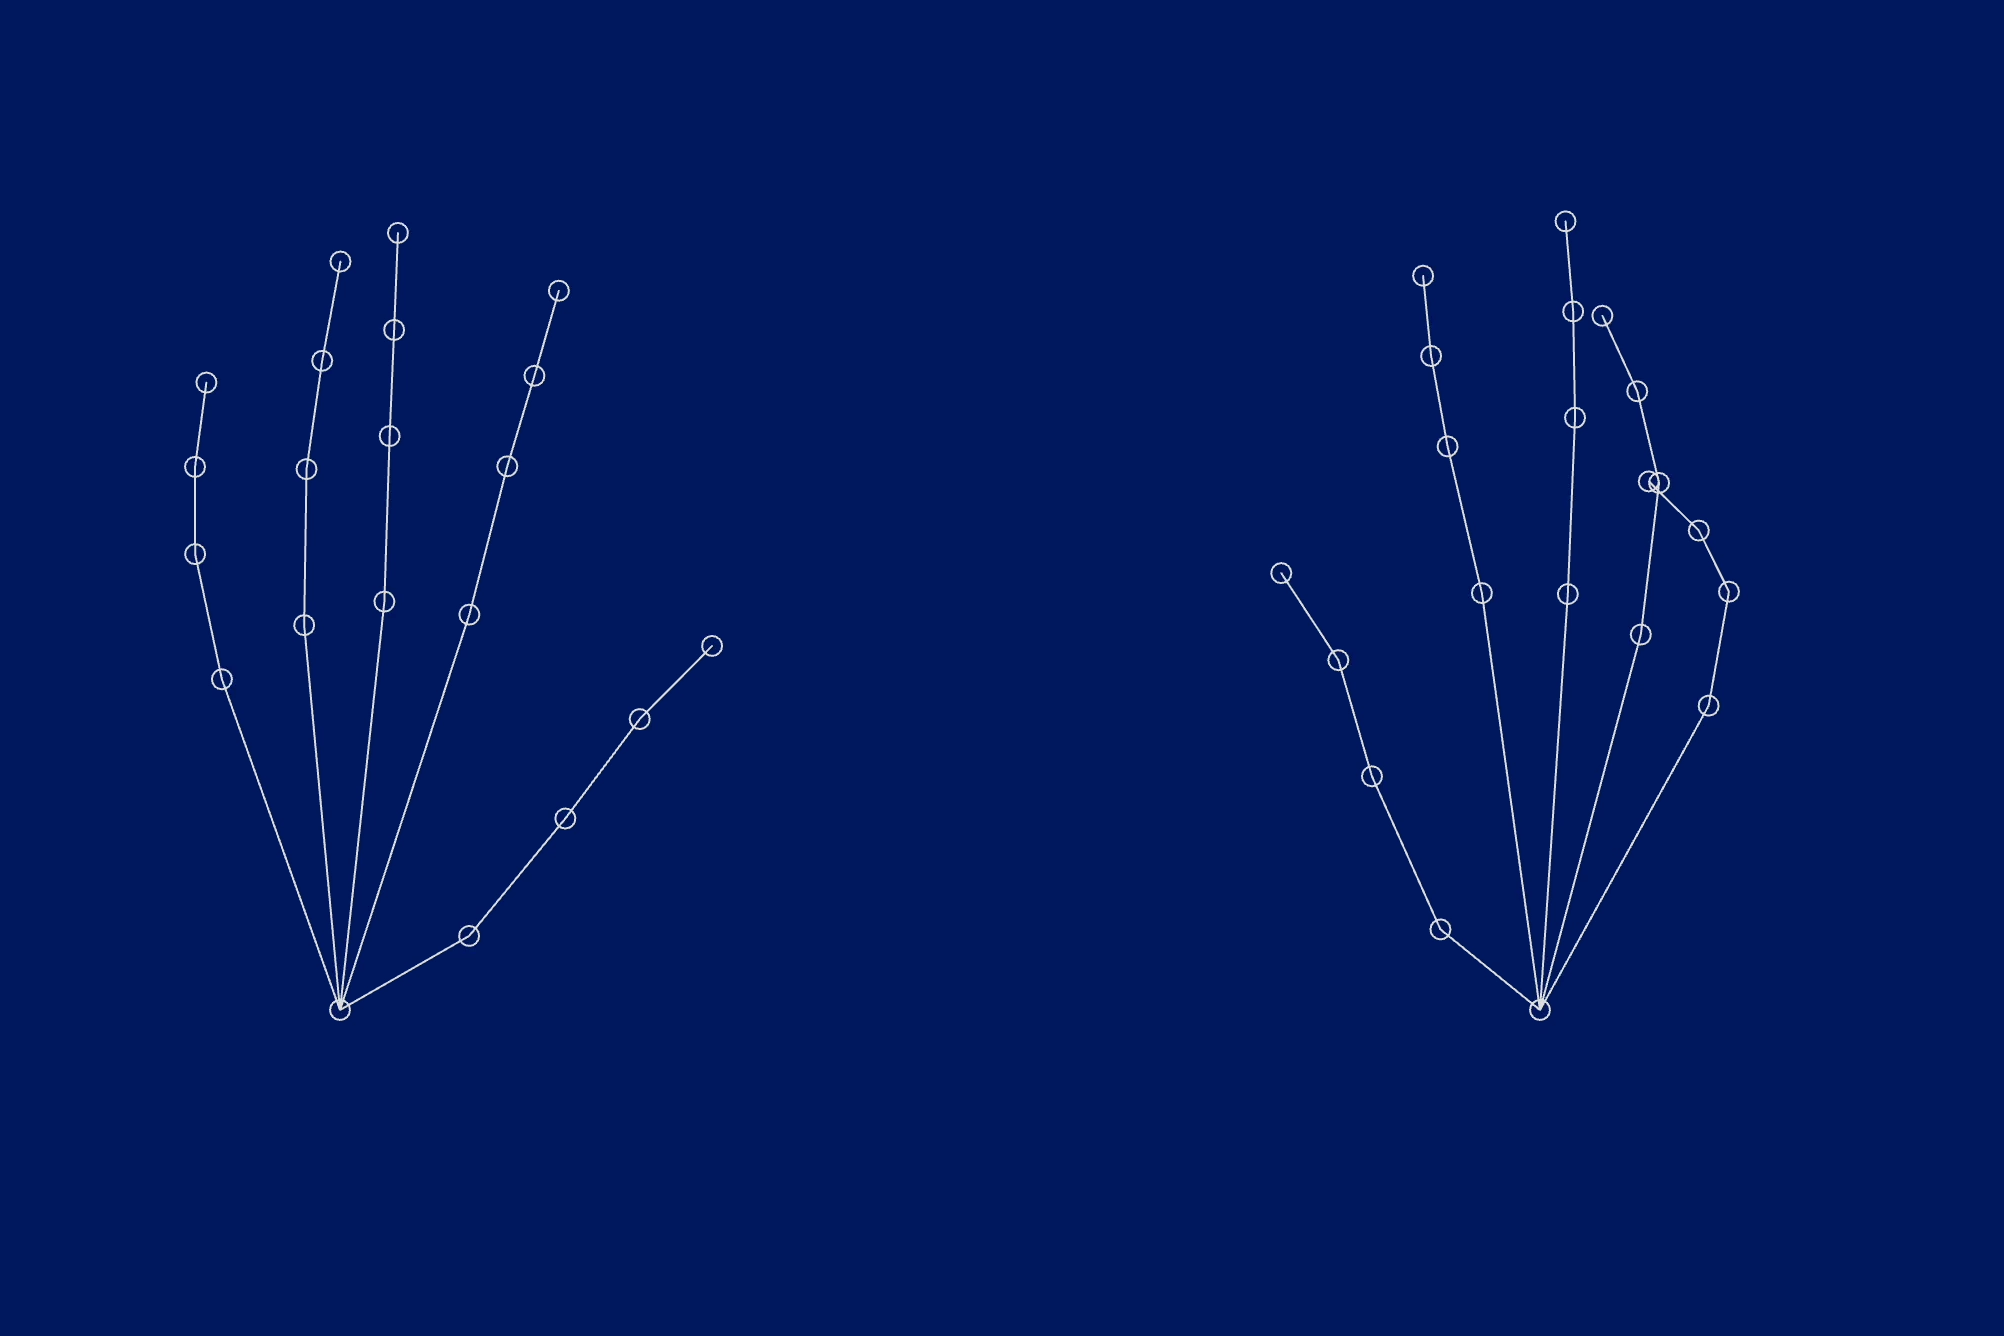
\includegraphics[keepaspectratio, width=7cm]{img/track_false.png}
    \caption{トラッキングに失敗しているとき}
    \label{fig:track_false}
  \end{minipage}
\end{figure}